% Options for packages loaded elsewhere
\PassOptionsToPackage{unicode}{hyperref}
\PassOptionsToPackage{hyphens}{url}
%
\documentclass[
  11pt,
  dvipsnames]{article}
\usepackage{amsmath,amssymb}
\usepackage{lmodern}
\usepackage{iftex}
\ifPDFTeX
  \usepackage[T1]{fontenc}
  \usepackage[utf8]{inputenc}
  \usepackage{textcomp} % provide euro and other symbols
\else % if luatex or xetex
  \usepackage{unicode-math}
  \defaultfontfeatures{Scale=MatchLowercase}
  \defaultfontfeatures[\rmfamily]{Ligatures=TeX,Scale=1}
\fi
% Use upquote if available, for straight quotes in verbatim environments
\IfFileExists{upquote.sty}{\usepackage{upquote}}{}
\IfFileExists{microtype.sty}{% use microtype if available
  \usepackage[]{microtype}
  \UseMicrotypeSet[protrusion]{basicmath} % disable protrusion for tt fonts
}{}
\makeatletter
\@ifundefined{KOMAClassName}{% if non-KOMA class
  \IfFileExists{parskip.sty}{%
    \usepackage{parskip}
  }{% else
    \setlength{\parindent}{0pt}
    \setlength{\parskip}{6pt plus 2pt minus 1pt}}
}{% if KOMA class
  \KOMAoptions{parskip=half}}
\makeatother
\usepackage{xcolor}
\IfFileExists{xurl.sty}{\usepackage{xurl}}{} % add URL line breaks if available
\IfFileExists{bookmark.sty}{\usepackage{bookmark}}{\usepackage{hyperref}}
\hypersetup{
  hidelinks,
  pdfcreator={LaTeX via pandoc}}
\urlstyle{same} % disable monospaced font for URLs
\usepackage[margin=1in]{geometry}
\usepackage{listings}
\newcommand{\passthrough}[1]{#1}
\lstset{defaultdialect=[5.3]Lua}
\lstset{defaultdialect=[x86masm]Assembler}
\usepackage{longtable,booktabs,array}
\usepackage{calc} % for calculating minipage widths
% Correct order of tables after \paragraph or \subparagraph
\usepackage{etoolbox}
\makeatletter
\patchcmd\longtable{\par}{\if@noskipsec\mbox{}\fi\par}{}{}
\makeatother
% Allow footnotes in longtable head/foot
\IfFileExists{footnotehyper.sty}{\usepackage{footnotehyper}}{\usepackage{footnote}}
\makesavenoteenv{longtable}
\usepackage{graphicx}
\makeatletter
\def\maxwidth{\ifdim\Gin@nat@width>\linewidth\linewidth\else\Gin@nat@width\fi}
\def\maxheight{\ifdim\Gin@nat@height>\textheight\textheight\else\Gin@nat@height\fi}
\makeatother
% Scale images if necessary, so that they will not overflow the page
% margins by default, and it is still possible to overwrite the defaults
% using explicit options in \includegraphics[width, height, ...]{}
\setkeys{Gin}{width=\maxwidth,height=\maxheight,keepaspectratio}
% Set default figure placement to htbp
\makeatletter
\def\fps@figure{htbp}
\makeatother
\setlength{\emergencystretch}{3em} % prevent overfull lines
\providecommand{\tightlist}{%
  \setlength{\itemsep}{0pt}\setlength{\parskip}{0pt}}
\setcounter{secnumdepth}{5}
\usepackage{setspace}
\usepackage{float}
\usepackage{fontspec}
\usepackage{subfig}
\usepackage[french]{babel}
\usepackage{csquotes}
\setmonofont{JetBrains Mono}[Contextuals=Alternate]
\floatplacement{figure}{H}
\lstset{ 
  language=python,                     % the language of the code
  basicstyle=\small\ttfamily, % the size of the fonts that are used for the code
  stepnumber=1,                   % the step between two line-numbers. If it is 1, each line
                                  % will be numbered
  numbersep=5pt,                  % how far the line-numbers are from the code
  backgroundcolor=\color{cyan!5},  % choose the background color. You must add \usepackage{color}
  showspaces=false,               % show spaces adding particular underscores
  showstringspaces=false,         % underline spaces within strings
  showtabs=false,                 % show tabs within strings adding particular underscores
  frame=single,                   % adds a frame around the code
  rulecolor=\color{black},        % if not set, the frame-color may be changed on line-breaks within not-black text (e.g. commens (green here))
  tabsize=2,                      % sets default tabsize to 2 spaces
  captionpos=b,                   % sets the caption-position to bottom
  breaklines=true,                % sets automatic line breaking
  breakatwhitespace=false,        % sets if automatic breaks should only happen at whitespace
  keywordstyle=\color{RoyalBlue},      % keyword style
  commentstyle=\color{Green},   % comment style
  stringstyle=\color{Orange},      % string literal style
}
\makeatletter
\renewcommand\paragraph{\@startsection{paragraph}{4}{\z@}%
        {-2.5ex\@plus -1ex \@minus -.25ex}%
        {1.25ex \@plus .25ex}%
        {\normalfont\normalsize\bfseries}}
\makeatother
\setcounter{secnumdepth}{4}
\hypersetup{
    colorlinks = true,
}
\ifLuaTeX
  \usepackage{selnolig}  % disable illegal ligatures
\fi
\usepackage[style=alphabetic,backend=biber]{biblatex}
\addbibresource{references.bib}

\author{}
\date{\vspace{-2.5em}}

\begin{document}

\onehalfspacing

\pagenumbering{gobble}

\begin{titlepage}
\vspace*{\fill}
\begin{center}
\LARGE{\textbf{Deep Image Prior}}\\
\Large{\textbf{Projet Modélisation 3MIC}}\\
\vspace*{1\baselineskip}
\Large{\textbf{Membres}}\\
PHAM Tuan Kiet\\
VO Van Nghia\\
\vfill % equivalent to \vspace{\fill}
\vspace*{\fill}
\today
\end{center}
\end{titlepage}

\newpage

\newpage
\pagenumbering{roman}
\tableofcontents
\addcontentsline{toc}{section}{\contentsname}

\listoffigures

\newpage
\pagenumbering{arabic}

\hypertarget{introduction}{%
\section{Introduction}\label{introduction}}

Le \protect\hyperlink{ruxe9seau-neuronal-convolutif}{Réseau neuronal convolutif} (en anglais \textbf{\emph{CNN}}) est actuellement l'une des techniques
les plus connues dans les problèmes de reconstruction d'image inverse.
Ils se sont avérés efficace dans un grand nombre de tâches, y compris le débruitage d'image,
la super-résolution d'image et la compression d'images avec perte.
Elle est un type de réseau de neurones artificiels acycliques (feed-forward),
dans lequel le motif de connexion entre les neurones est inspiré
par le cortex visuel des animaux.

La puissance de cette architecture est attribuée à sa capacité d'apprendre
à partir de nombreux grands ensembles d'images.
Cependant, \autocite{2007.02471,1711.10925} et de nombreux autres travaux ont démontré
que l'architecture d'un CNN peut agir comme un préalable suffisamment fort pour résoudre
\protect\hyperlink{les-probluxe8mes-inverses}{des problèmes inverses} comme la reconstruction d'image,
même sans étape d'apprentissage. Plus précisément, les réseaux non entrainés
fonctionnent bien pour le débruitage d'image \autocite{2007.02471},
l'acquisition comprimée \autocite{1806.06438} et même pour la reconstruction de vidéos \autocite{1910.01684}.

Dans ce travail, nous nous concentrerons sur la technique \textbf{\emph{Deep Image Prior}}.
Dans la partie suivante, nous allons examiner quelques exemples.
Puis, nous approfondissons le principe sous-jacent de celui-ci à travers l'exemple précédent.
Enfin, nous expérimenterons ce que nous venons de présenter ci-dessus
et ferons quelques études complémentaires.

Tout d'abord, nous clarifierons certaines terminologies.

\hypertarget{ruxe9seau-neuronal-convolutif}{%
\subsection{Réseau neuronal convolutif}\label{ruxe9seau-neuronal-convolutif}}

Un réseau neuronal est l'association d'objets élémentaires, les neurones formels, interconnectés
permettant la résolution de problèmes complexes
tels que la reconnaissance des formes ou le traitement du langage naturel,
grâce à l'ajustement des coefficients de pondération dans une phase d'apprentissage.
Les principaux réseaux se distinguent par l'organisation du graphe (en couches, complets, \(etc,\)),
c'est-à-dire leur architecture, son niveau de complexité
(le nombre de neurones, présence ou non de boucles de rétroaction dans le réseau)
par le type des neurones (leurs fonctions de transition ou d'activation)
et enfin par l'objectif visé: apprentissage supervisé ou non, optimisation,
systèmes dynamiques, \(etc.\)

Le premier modèle mathématique et informatique du neurone biologique est proposé par Warren McCulloch et Walter Pitts
Dans le modèle de McCulloch et Pitts, à chaque entrée est associé une valeur numérique appelé le poids synaptique.
Donc, nous pouvons écrire le neurone formel comme un modèle qui se caractérise par
un état interne \(s\) , des signaux d'entrée \(x_{1}\), \dots, \(x_{p}\) avec les poids synaptique associé
\(\alpha_{1}\), \dots, \(\alpha_{p}\) et une fonction d'activation
\[ s=h(x_{1},\dots,x_{p})=\phi(\alpha_{0} + \sum_{j=1}^{p} \alpha_{j}x_{j}) = \phi(\alpha_{0} + \alpha' x)\]

La fonction d'activation opère une transformation d'une combinaison affine
des signaux d'entrée, \(\alpha_{0}\), terme constant, étant appelé le biais du neurone.
Cette combinaison affine est déterminée par un vecteur de poids
\([\alpha_{0},\dots,\alpha_{p}]\) associé à chaque neurone et dont les valeurs sont estimées dans la phase d'apprentissage.
Ils constituent la mémoire ou connaissance répartie du réseau.

Un réseau de neurones convolutifs ou réseau de neurones à convolution
est un type de réseau de neurones artificiels, dont architecture est formée par
un empilement de couches (les combinaisons des neurones formels) de traitement:

\begin{itemize}
\tightlist
\item
  La couche de convolution (CONV)
\item
  La couche de pooling (POOL)
\item
  La couche d'activation
\item
  La couche ``entièrement connectée'' (FC)
\item
  La couche de perte (LOSS)
\end{itemize}

\hypertarget{les-probluxe8mes-inverses}{%
\subsection{Les problèmes inverses}\label{les-probluxe8mes-inverses}}

Les problèmes inverses peuvent être formulés comme la tâche d'optimisation avec la formule:
\[x^* = min_{x}E(x;x_{0}) + R(x)\]

Le réseau neuronal convolutionnel va décoder et générer une fonction de type:
\[x = f_{\theta}(z)\]
qui correspond bien aux données. La fonction va lier un vecteur qui est donné au hasard avec une image \(x\).
La méthode est sélectionnée spécifiquement pour chaque application.

\hypertarget{deep-image-prior}{%
\section{Deep Image Prior}\label{deep-image-prior}}

\hypertarget{principles}{%
\subsection{Principles}\label{principles}}

La technique \textbf{\emph{Deep Image Prior}} a fait une percée dans la dans le contexte
de problèmes inverses mal posés. Le réseau est connu pour le reconstruction d'image sans
étape d'apprentissage. Nous allons étudier les principles dedans et comment cette technique fonctionne.

Normalement, le \textbf{\emph{Deep learning}} aborde un problème par deux étapes. Premièrement, c'est l'étape d'apprentissage.
Dans cette étape, le paramètre de réseau est optimisé par minimiser un approprié fonction de perte à partir de
un grande ensemble de données. Puis, les nouvelles données est traité dans le réseau pour résoudre le problème.
Néanmoins, la technique \textbf{\emph{Deep Image Prior}} est basé seulement sur une seul point de données \(y^\gamma\). C'est-à-dire
la technique est d'entrainer un réseau avec son paramètre par minimiser la fonction de perte: \(\min_{\xi} \mid\mid A\varphi_\xi(z) - y^\gamma \mid\mid^2\).

Le resultat sur le réseau de \textbf{\emph{Deep Prior}} utilise le feed-forward architecture qui commence par:

\begin{center} $x^0 = z$    et    $x^{k+1} = \phi (W_k x^k + b_k)$ for $k = 0,...,L-1$  \end{center}

Donc, les résultats obtenues sont \(\varphi_\xi(z) = x^L\) avec les paramètres \(\xi = \{W_0,...,W_{L-1},b_0,...,b_{L-1}\}\)
Pour la technique \textbf{\emph{Deep Image Prior}}, il n'y a pas d'étape d'apprentissage. Donc, \(\xi\) n'est pas fixé.
La solution pour le problème inverse est \(x=\varphi_\xi(z)\) avec z fixé. La technique vise à paramétriser
la solution avec \(\xi\).

\hypertarget{muxe9thode}{%
\subsection{Méthode}\label{muxe9thode}}

Dans ce projet, nous cherchons à comprendre le fonctionnement de cette technique
en utilisant le prieur implicitement capturé par le choix d'une structure de réseau de générateurs particulière.
Nous avons mis un paramétrage \(x = f_\theta(z)\) avec \(x\) est un image de \(R^{3xHeightxWidth}\) (une image colorée de taille
Height x Width pixels a chaque pixel un combinaison de 3 couleurs rouge, vert et bleu).
Ici, \(\theta\) sont des paramètres du réseau.

\hypertarget{les-aspects-techniques}{%
\section{Les aspects techniques}\label{les-aspects-techniques}}

Dans cette partie, nous proposons un résumé des différents aspects techniques de la techniques de DIP(ou Deep Image Prior).
Cela nous aidera à établir une connexion entre les mathématiques et l'informatique plus facilement
et fournira également des informations supplémentaires sur ``Deep Image Prior''.

\hypertarget{le-code}{%
\subsection{Le code}\label{le-code}}

Tout d'abord, nous entrons dans le code. Comme indiqué ci-dessus, nous avons essayé de réécrire le code dans \autocite{1711.10925}.
Étant donné que chaque problème nécessite un modèle différent, nous nous concentrons uniquement sur le modèle de débruitage
(bien que notre code devrait fonctionner avec la plupart des modèles de cet article).

Outre la motivation de mieux comprendre le code, il y a
quelques raisons techniques à nos motivations pour un réimplémentation.
Nous le réécrivons à l'aide de TensorFlow, et nous ajoutons également
des métriques supplémentaires pour mesurer le PSNR entre l'image
débruitée et l'image bruité et le PSNR entre l'image débruitée etl'image originale.

\hypertarget{le-moduxe8les}{%
\subsection{Le modèles}\label{le-moduxe8les}}

Nous avons fait une architecture CNN très typique. Bien que le modèle dans \autocite{1711.10925}
soit plus profond et ait beaucoup plus de couches, il a toujours le même groupe de couches
qu'un auto-encodeur (\protect\hyperlink{duxe9codage-et-encodage}{décodage et encodage}) avec sauts de connexions. Notons qu'un décodeur soit suffit,
nous avons aussi essayé d'écrire seulement un décodeur pur.

L'entrée du modèle est un tenseur de forme \passthrough{\lstinline![batch\_size, image\_height, image\_width, 32]!} où \passthrough{\lstinline!batch\_size!} vaut 1 dans notre cas. 32 est le nombre de canaux (caractéristiques) qui seront expliqués plus tard. Sa sortie est un tenseur avec une forme de \passthrough{\lstinline![batch\_size, image\_height, image\_width, 3]!} qui pourrait être affiché comme une image (3 canaux car nous avons une image RGB (Red-Green-Blue)).

\hypertarget{duxe9codage-et-encodage}{%
\subsection{Décodage et encodage}\label{duxe9codage-et-encodage}}

Dans cette partie, nous travaillons sur la première architecture de CNN que nous avons fait.
Elle est l'architecture ayant toujours un étape d'auto-encodeur.

\begin{figure}

{\centering \subfloat[original\label{fig:compare-with-edge-1}]{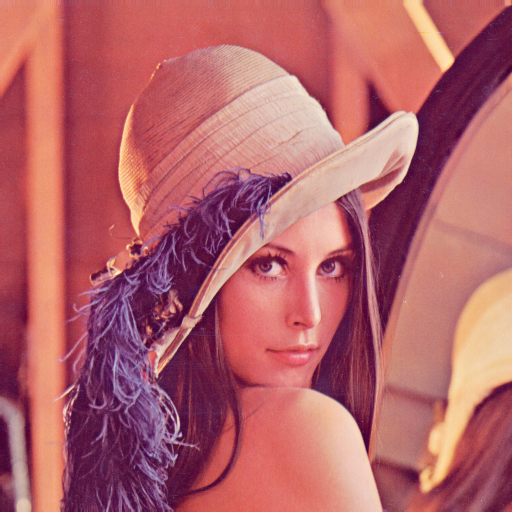
\includegraphics[width=0.5\linewidth]{../res/edge/lena} }\subfloat[bord\label{fig:compare-with-edge-2}]{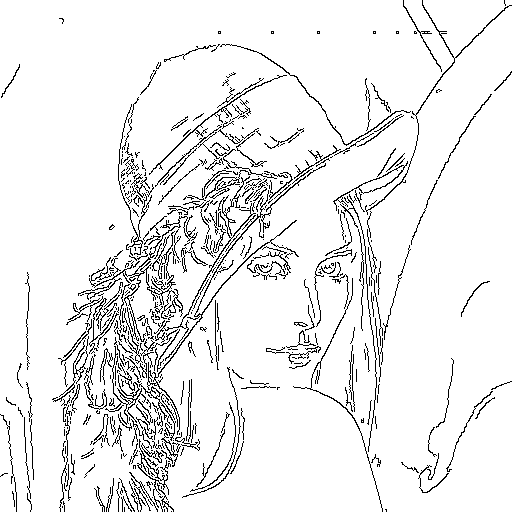
\includegraphics[width=0.5\linewidth]{../res/edge/lena_edge} }

}

\caption{La détection de bord}\label{fig:compare-with-edge}
\end{figure}

Le décodage est un processus d'extraction de caractéristiques d'une image.
Sur le côté opposé, l'encodeur collectera les caractéristiques des décodeurs
et reconstruira l'image. Les caractéristiques peuvent être n'importe quoi,
varient des bords (\ref{fig:compare-with-edge}), de la couleur à la résolution.

Dans notre cas, le nombre de 32 de l'architecture signifie que nous capturons 32
caractéristiques différentes à partir d'une image bruité pour reconstruire
l'image d'origine. En fait, on pourra reconstruire l'image seulement si le nombre
de paramètre du réseau est supérieur au nombre de pixels dans l'image. La technique
\textbf{\emph{Deep Image Prior}} ne comprend pas d'étape d'apprentissage. Donc, les décodeurs
considéreront le bruit comme une caractéristique et le captureront.
Cela explique pourquoi si nous répétons le processus trop souvent, l'image de
sortie tendra vers l'image bruité ou vers un résultat que nous n'attendons pas.

Sous le capot, le décodeur est construit à partir d'opérations convolutives.
En parcourant chaque pixel et en appliquant le noyau convolutif, nous pourrions extraire
les fonctionnalités souhaitées. L'illustration d'une opération convolutive en image avec un \(2 x 2\) kernel
peut être vue comme suit:
\[\left(\begin{bmatrix}
  0 & 0 & 0 & 0 & 0\\
  0 & a & b & c & 0\\
  0 & d & e & f & 0\\
  0 & g & h & j & 0\\
  0 & 0 & 0 & 0 & 0\\
\end{bmatrix}
\begin{bmatrix}
  1 & 1\\
  1 & 1\\
\end{bmatrix}\right) =
\begin{bmatrix}
  a & a+b & b+c & c\\
  a+d & a+b+d+e & b+c+e+f & c+f\\
  d+g & d+e+g+h & e+f+h+j & f+j\\
  g & g+h & h+j & j\\
\end{bmatrix}
\]

\hypertarget{la-sortie}{%
\subsection{La sortie}\label{la-sortie}}

Pour mieux comprendre, nous avons bouclé le processus 6000 fois. Nous étudions
les différences entre chaque étape de boucle pour avoir un mieux vue de notre
algorithm.

Voici notre image de test:

\begin{figure}

{\centering \subfloat[original\label{fig:noisy-original-image-1}]{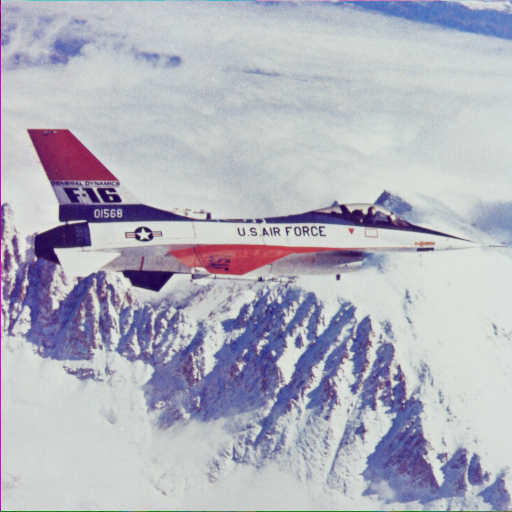
\includegraphics[width=0.25\linewidth]{../res/denoising/input} }\subfloat[bruyant\label{fig:noisy-original-image-2}]{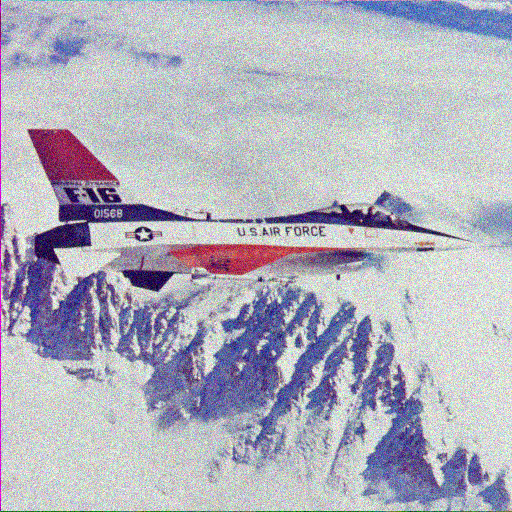
\includegraphics[width=0.25\linewidth]{../res/denoising/noisy} }

}

\caption{L'image originale et l'image bruité}\label{fig:noisy-original-image}
\end{figure}

Et le résultat que nous obtenons:

\begin{figure}

{\centering \subfloat[1\label{fig:model-epoch-output-1}]{
\includegraphics[width=0.25\linewidth]{../res/denoising/epoch_0} }\subfloat[1000\label{fig:model-epoch-output-2}]{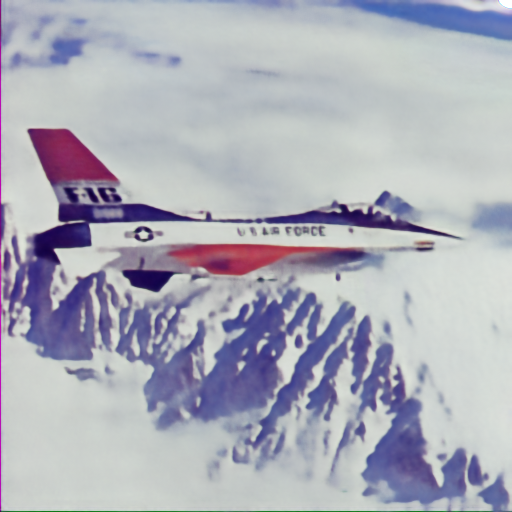
\includegraphics[width=0.25\linewidth]{../res/denoising/epoch_999} }\subfloat[3000\label{fig:model-epoch-output-3}]{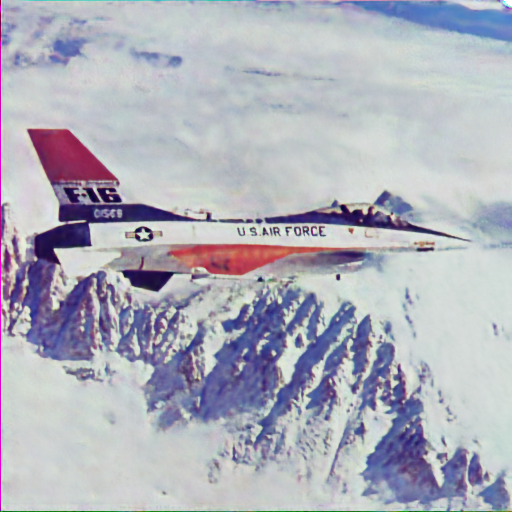
\includegraphics[width=0.25\linewidth]{../res/denoising/epoch_2999} }\subfloat[6000\label{fig:model-epoch-output-4}]{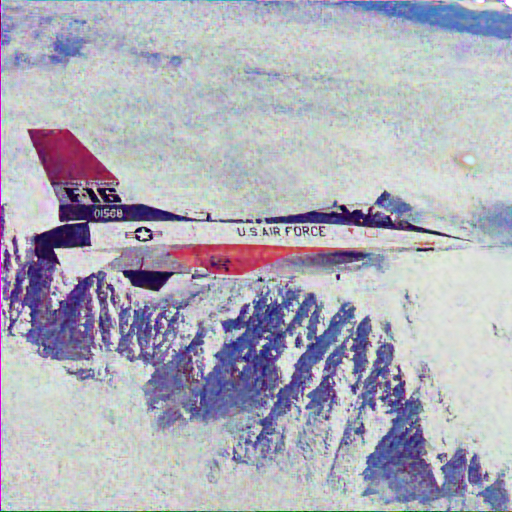
\includegraphics[width=0.25\linewidth]{../res/denoising/epoch_5999} }

}

\caption{La sortie de l'epoch}\label{fig:model-epoch-output}
\end{figure}

Nous pouvions voir clairement les différences entre chaque epoche. Cela pourrait s'expliquer comme suit:

\begin{itemize}
\tightlist
\item
  A la première époque, l'entrée est un bruit aléatoire et le modèle est initialisé avec des poids aléatoires. Nous voyons donc une image aléatoire, qui n'est pas liée à la sortie souhaitée.
\item
  Vers la 1000e époque, les décodeurs à l'intérieur du modèle commencent à s'ajuster pour extraire les caractéristiques de l'image bruité. Premièrement, ils extraient les plus importants comme le bord, la couleur, la résolution, \(etc.\)
\item
  A la 3000ème époque, les décodeurs et encodeurs sont désormais capables d'extraire toutes les caractéristiques souhaitées et de reconstruire une image de sortie comme on le voit dans \ref{fig:model-epoch-output}.
\item
  Plus nous bouclons le processus, plus il y a de parties extraites et des caractéristiques indésirables comme le bruit sont également incluses. Par conséquent, nous voyons une image assez proche de l'image bruyante (\ref{fig:noisy-original-image}).
\end{itemize}

Pour une vue plus scientifique, ce sont les métriques que nous avons utilisées lors de l'itération de ce modèle.

D'après la figure \ref{fig:model-psnr}, il y a une tendance croissante dans le PSNR entre l'image débruitée et l'image bruyante. D'autre part, le PSNR entre celui-ci et l'image d'origine atteint son apogée vers 3000 epoches et commence à diminuer par la suite. Cela correspond à ce que nous avons vu auparavant en comparant différentes sorties avec nos yeux.

\begin{figure}

{\centering \subfloat[originale\label{fig:model-psnr-1}]{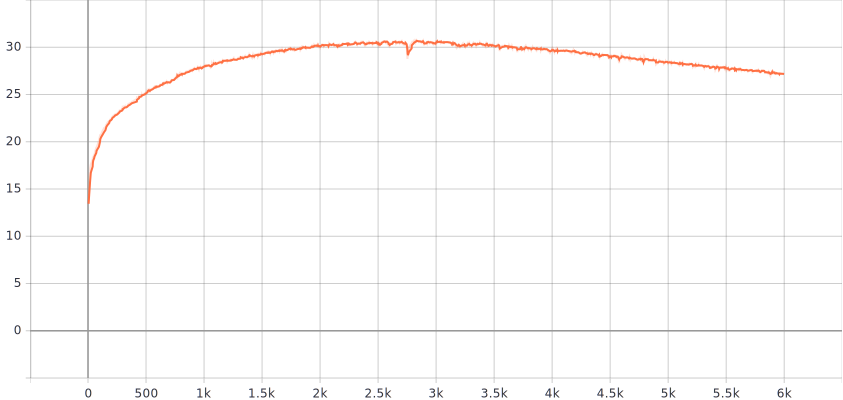
\includegraphics[width=0.5\linewidth]{../res/denoising/psnr_original} }\subfloat[bruité\label{fig:model-psnr-2}]{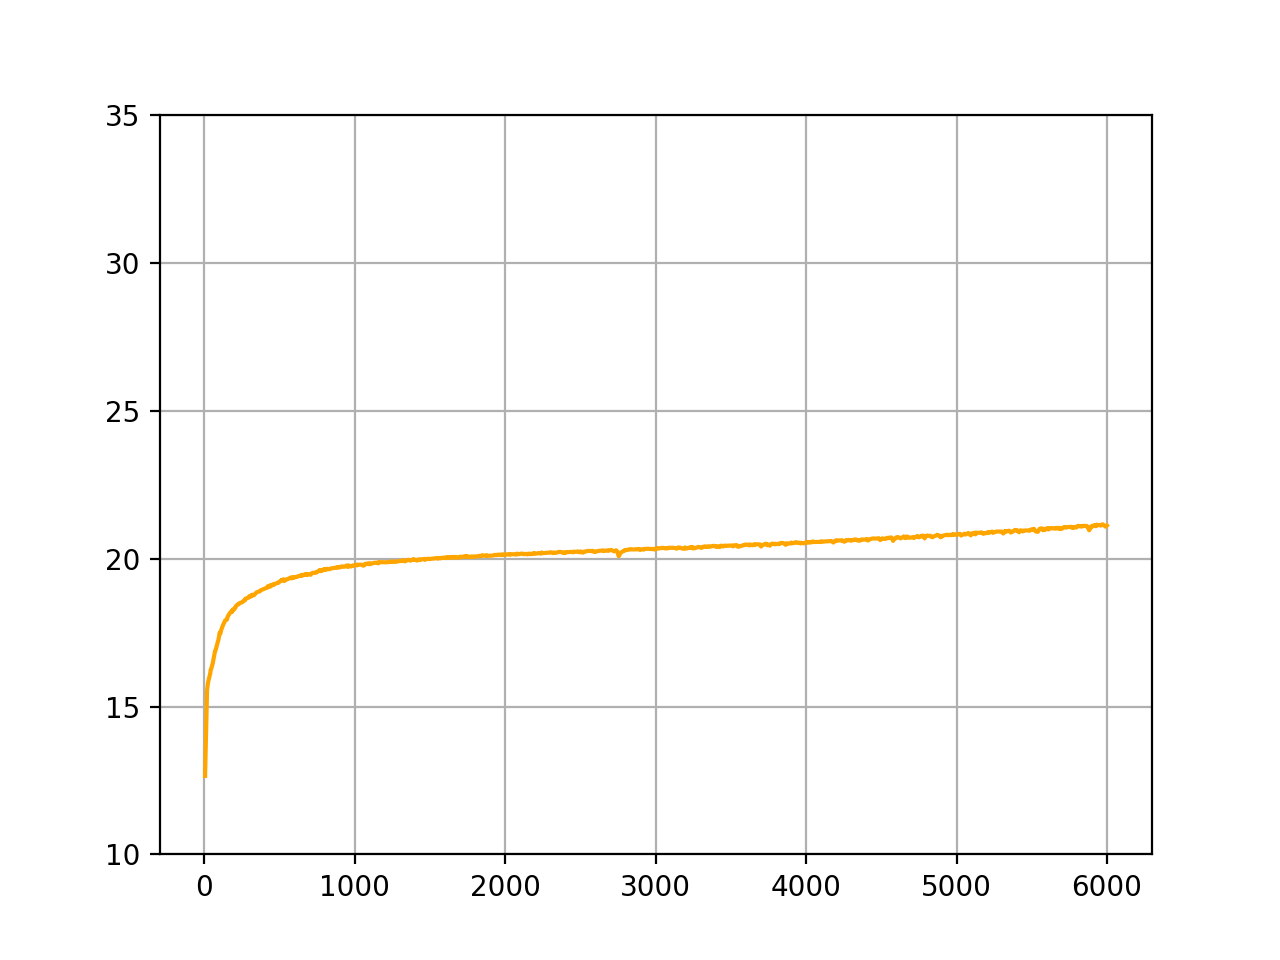
\includegraphics[width=0.5\linewidth]{../res/denoising/psnr_noisy} }

}

\caption{Le PSNR entre l'image débruitée et l'image}\label{fig:model-psnr}
\end{figure}

\hypertarget{conclusion}{%
\section{Conclusion}\label{conclusion}}

Dans ce projet, nous avons étudié d'un nouvelle technique de traitement d'image.
Cette technique n'a pas besoin quantité massive de données (un seul point de données \(y^\gamma\))
ni un modèle pre-entrainé (sans étape d'apprentissage). Nous avons testé différents modèles et données
pour avoir un meilleur vue de fonctionnement de nos architecture et de la technique DIP.
Ce que nous avons obtenu nous montre des résultats prometteurs.
\newpage

\printbibliography

\end{document}
